\documentclass[sigconf, nonacm]{acmart}

% School submission settings
\setcopyright{none}
\renewcommand\footnotetextcopyrightpermission[1]{}
\pagestyle{plain}
\acmDOI{}
% Color for figure borders
\definecolor{bordergray}{gray}{0.3}

% Image box command
\newcommand{\imgbox}[1]{%
  \begingroup
  \setlength{\fboxsep}{1pt}%
  \setlength{\fboxrule}{0.2pt}%
  \fcolorbox{bordergray}{white}{%
    \begin{minipage}{\dimexpr\linewidth-2\fboxrule\relax}
      \centering
      #1
    \end{minipage}
  }%
  \endgroup
}

\usepackage{subcaption}
\usepackage{float}

% Figures directory
\graphicspath{{./images/}}

\pagestyle{plain} 
\makeatletter
\let\@shorttitle\@empty
\let\@shortauthors\@empty
\makeatother
\pagestyle{plain}


\begin{document}

\title[]{Sentiment Analysis of the Philippine News Using Natural Language Processing}

\author{Jose Marie G.\ Lim}
\affiliation{%
  \institution{Guimaras State University}
  \department{College of Science and Technology}
  \city{Jordan, Guimaras}
  \country{Philippines}
}

\begin{abstract}
The speed and volume of modern online journalism make systematic monitoring of news coverage increasingly difficult through manual methods. Articles are continuously published across multiple digital outlets, creating a fragmented information landscape where identifying patterns in tone and coverage requires automated support. This paper presents PH Eye, an end-to-end web-based analytics platform is designed to ingest, process, and visualize news articles from major Philippine news sources using continuous scheduled collection. The system integrates automated web scraping, text preprocessing, lexicon-based sentiment classification, and named entity extraction to transform raw articles into structured insights. PH Eye aggregates news from seven online outlets into a centralized interface that provides sentiment-labeled article streams, entity-level sentiment scoring, and cross-source comparison tools. The platform also includes visualization components such as trend dashboards and Pearson correlation heatmaps to reveal how sentiment patterns converge or diverge across sources over time. Experiments conducted on a seven-day collection of news articles demonstrate the system’s ability to surface temporal tone shifts and highlight differences in coverage among outlets. The study contributes an end-to-end automated pipeline and interactive monitoring platform for exploring sentiment and entity trends in Philippine digital news, providing researchers and analysts with tools to examine large-scale media patterns more efficiently.
\end{abstract}

\keywords{Natural Language Processing, continuous monitoring, sentiment analysis, web-based system, Philippine online news, named entity recognition, Pearson correlation}

\maketitle

\section{Introduction}
Online news has become a primary channel through which audiences encounter public issues, and the speed and volume of online publishing makes systematic monitoring challenging for students, researchers, and media observers \cite{datareportal}. In practice, even motivated readers quickly face a familiar problem: by the time one topic is reviewed, dozens of new stories have already been published across multiple outlets. This creates a gap between the pace of publishing and the pace of careful interpretation.

Beyond factual content, the \emph{tone} and \emph{framing} of headlines and narratives influence what readers notice and how they interpret events \cite{entman1993framing}. Agenda-setting theory further argues that sustained coverage can shape which issues are perceived as important \cite{mccombs1972agenda}. For Philippine news in particular, where public attention can shift rapidly due to elections, disasters, and policy events, it is useful to have tools that support consistent monitoring without replacing human judgment.

Manual content analysis can provide rich interpretation, but it does not scale well across multiple outlets and continuous publication cycles. A practical alternative is to treat NLP outputs as \emph{signals}: a way to compress large volumes of text into summaries that help analysts decide what to read next. In this view, the goal is not to produce a final verdict on intent or bias, but to surface patterns that can guide deeper qualitative review.

This capstone project addresses that need by building PH Eye, an automated pipeline for collecting and summarizing sentiment signals in Philippine online news. The system (1) gathers articles from selected sources using browser automation \cite{playwright}, (2) normalizes and preprocesses text, (3) estimates sentiment polarity using the VADER rule-based lexicon approach \cite{hutto2014vader}, and (4) extracts named entities using spaCy \cite{spacy} to support entity-level aggregation. Together, these steps make it possible to monitor changes in coverage tone over time, compare outlets within a fixed window, and drill down from aggregates to the underlying articles \cite{pang2008opinionmining,liu2012sentiment}.

In addition to the NLP pipeline, PH Eye is implemented as a deployed end-to-end system. A web user interface built with Next.js \cite{nextjs} is hosted on Vercel \cite{vercel} to provide an accessible dashboard and article views. The backend exposes a REST API using FastAPI \cite{fastapi} and runs in Docker containers \cite{docker} to support repeatable deployment. Collection and analysis are executed as scheduled background jobs using Celery \cite{celery} with Redis \cite{redis} as a broker/cache, while results are stored in a Supabase-managed PostgreSQL database \cite{supabase,postgresql}. This architecture supports continuous collection and analysis while keeping the monitoring workflow centered on an interactive UI.

To keep claims concrete and comparable, this paper reports results using a 7-day snapshot of the system database. The snapshot is used to demonstrate end-to-end behavior (collection, scoring, aggregation, and visualization) and to illustrate how sentiment distributions, temporal trends, and cross-source co-movement can be summarized in a compact dashboard-style workflow.

The rest of the paper is organized as follows: Section~2 describes the methodology; Section~3 presents results and discussion; and Section~4 concludes with limitations and future work.

\section{Methodology}
PH Eye consists of four stages: (i) automated collection, (ii) preprocessing and normalization, (iii) NLP analysis, and (iv) storage and visualization. The overall workflow follows a pipeline structure in which raw news articles are first collected from external sources, then preprocessed and analyzed using NLP techniques, and finally stored and served through an interactive web interface for visualization and exploration.

Articles are collected from selected Philippine news outlets using Playwright \cite{playwright} to handle JavaScript-rendered pages.

\subsection{System Architecture and Deployment}

Figure~\ref{fig:architecture} summarizes the system architecture. The system is designed as an end-to-end pipeline for automated news collection, processing, and visualization. The frontend is a Next.js web application deployed on Vercel \cite{nextjs,vercel}. The backend provides a REST API implemented in FastAPI \cite{fastapi} and deployed using Docker \cite{docker}. To support continuous scheduled collection and analysis, background tasks are executed using Celery \cite{celery} with Redis \cite{redis} as a message broker and cache. Articles and analysis outputs are persisted in a Supabase (PostgreSQL) database \cite{supabase,postgresql}.

\begin{figure}[h]
  \centering
  \imgbox{\includegraphics[width=\linewidth]{architecture.png}}
  \caption{PH Eye system architecture: Next.js frontend (Vercel), FastAPI backend (Docker), Celery worker/beat with Redis, Supabase (PostgreSQL) storage, and external news sources.}
  \label{fig:architecture}
\end{figure}

The system follows a three-layer design. The Next.js frontend renders dashboards and either calls the FastAPI backend for analytics endpoints (/ml/*, /articles/*) or reads directly from Supabase for selected listings. The FastAPI backend handles application logic, interacts with Supabase for data persistence, and uses Redis for caching and task queueing. Celery Beat schedules scraping tasks, while Celery workers execute scraping and NLP processing, with results stored in Supabase tables (e.g., articles, analyzed articles, and scraping logs).

\subsection{Data Sources and Inclusion Criteria}
The dataset consists of English-language news articles collected from major Philippine online outlets (GMA News Online, Rappler, Inquirer.net, Manila Times, Manila Bulletin, Philstar, and SunStar). For each article, the system retains the main textual content (title and body) and core metadata (source, canonical URL, publication date, and category when available). Non-news elements such as advertisements, navigation boilerplate, embedded widgets, and comment sections are excluded during extraction. To reduce subjective writing styles in the dataset, the collection pipeline applies source-specific URL/path and category filtering rules intended to exclude opinion/editorial pages; any residual opinion-style articles that bypass filtering are treated as noise and are not the analytical focus of the study.

\subsection{Collection and Normalization}
For each target source, the scraper retrieves pages using a combination of HTTP fetching and headless browser automation (Playwright) for JavaScript-rendered content. After the article content renders, the pipeline extracts the canonical URL, title, and body text. Duplicate detection is performed by canonical URL checks against the database to avoid redundant ingestion. Extracted text is normalized through whitespace standardization and boilerplate removal to ensure that downstream NLP steps receive consistent input across heterogeneous site templates.

\subsection{NLP Analysis}
Sentiment polarity is computed using the VADER lexicon-based approach \cite{hutto2014vader}. Because full-length news articles can dilute polarity when analyzed as a single block, the implementation applies a long-form scoring strategy: the article is segmented into manageable text chunks and aggregated using weighted components (title, leading portion, and remaining body). Each article produces a compound sentiment score in the range $[-1,1]$ and a categorical label (positive, neutral, or negative) using fixed thresholds ($\geq 0.05$ for positive, $\leq -0.05$ for negative, otherwise neutral). This design was selected to support near real-time processing on limited local hardware while maintaining interpretable outputs.

Named entities are extracted using spaCy \cite{spacy} to identify persons, organizations, and geographic entities \cite{nadeau2007ner}. Entity outputs are normalized and aggregated to support frequency ranking and entity-level sentiment summaries within the selected analysis window.


\subsection{Storage Model and Evaluation Window}
Processed articles and analysis outputs are stored in a Supabase-managed PostgreSQL database \cite{supabase,postgresql} to support reproducible queries and aggregation. The system persists (i) normalized article records (URL, title, publication time, cleaned text, and source), (ii) per-article sentiment outputs and model metadata, and (iii) operational scraping logs to track coverage, execution status, and failures. For this paper, results are reported using a fixed 7-day snapshot of the database, enabling daily summaries, cross-source comparisons, correlation analysis, and entity-level breakdowns within a consistent observation window.


\section{Results and Discussion}
This section summarizes results from the 7-day snapshot using sentiment distributions, temporal trends, and cross-source correlation analysis.

\subsection{News Dashboard/Home Screen}
Figure~\ref{fig:homescreen} displays recently scraped articles grouped by source (GMA, Rappler, Inquirer, Manila Times, Philstar, Sunstar, and Manila Bulletin). Each source block presents article cards containing the headline, publication date, and sentiment label. A View All action per source opens a dedicated source-specific listing for deeper browsing. This layout supports quick cross-source monitoring while preserving organized presentation.

\begin{figure}[h]
  \centering
  \imgbox{\includegraphics[width=\linewidth]{images/hompage.png}}
  \caption{PH eye Home Screen displays news from 7 sources.}
  \label{fig:homescreen}
\end{figure}



\subsection{Overall distribution and temporal trends}
Figure~\ref{fig:trends} presents the weekly distribution of sentiment classifications across the collected news sources.
 Across the 7-day snapshot ($n=1687$ articles; $241$ articles/day on average), positive sentiment dominated the collected articles (57.9\%), followed by negative sentiment (39.0\%), while neutral classifications remained minimal. This skew suggests that polarity signals are influenced by the mix of topics in the window and by the behavior of a lexicon-based analyzer in news contexts \cite{hutto2014vader}. Figure~\ref{fig:trends} illustrates that sentiment counts fluctuate with publication volume, which is useful for spotting periods where negative or positive coverage spikes for investigation via the underlying articles and entity summaries.
\begin{figure}[h]
  \centering
  % width is set to \linewidth inside the box for perfect centering
  \imgbox{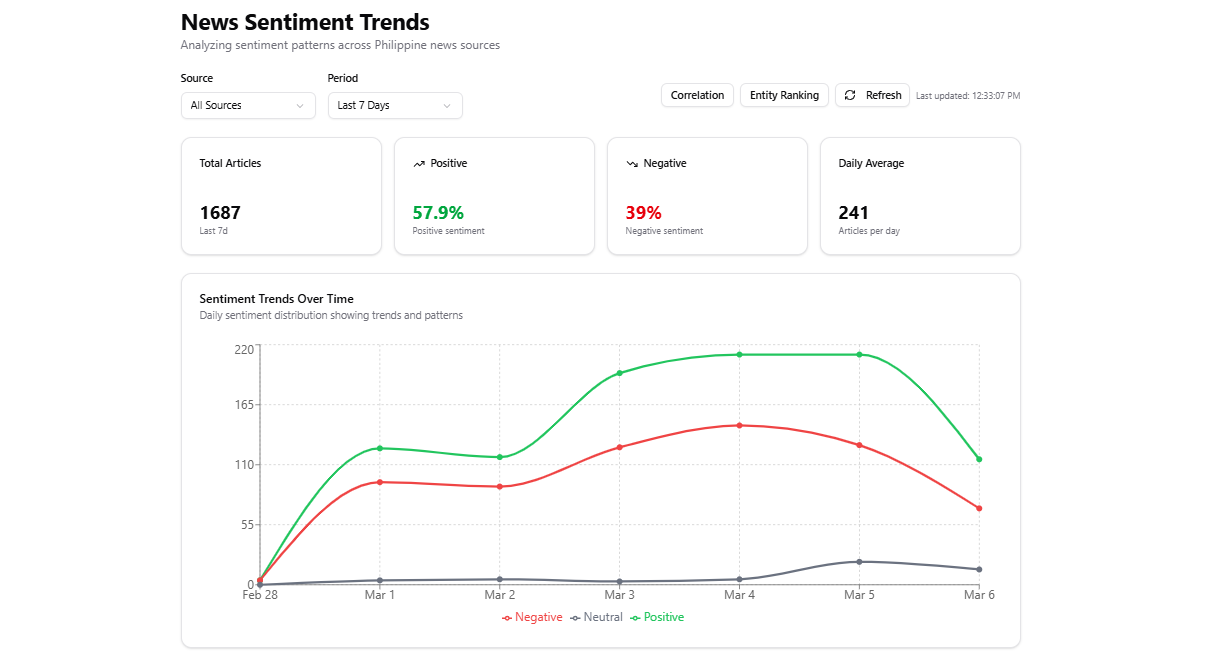
\includegraphics[width=\linewidth]{weekly-sentiment-trends.png}}
  \caption{Weekly sentiment trends across sources (7-day snapshot).}
  \label{fig:trends}
\end{figure}
~\ref{tab:gma-avg} lists the daily VADER average score for GMA (see Figure~\ref{fig:correlation}(\subref{fig:correlation-gma})).
\begin{table}[h]
  \caption{GMA daily average sentiment (VADER).}
  \label{tab:gma-avg
\subsection{Pearson Correlaton Matrix}
Figure~\ref{fig:correlation-heatmap} focuses on the statistical alignment between the seven news sources. It features the Source Correlation Matrix, a heatmap visualization based on Pearson correlation coefficients computed from daily sentiment averages (Equation~\ref{eq:pearson}).

\begin{equation}\label{eq:pearson}\small
r_{XY}=\frac{\sum_{i=1}^{n}(x_i-\bar{x})(y_i-\bar{y})}{\sqrt{\sum_{i=1}^{n}(x_i-\bar{x})^2}\sqrt{\sum_{i=1}^{n}(y_i-\bar{y})^2}}
\end{equation}

Here, $x_i$ denotes the daily average sentiment score for source $X$ on day $i$, $y_i$ denotes the daily average sentiment score for source $Y$ on day $i$, and $\bar{x}$ and $\bar{y}$ are the mean daily sentiment scores over the observation window. The value $n$ is the number of paired days included in the computation; when either source has no articles on a given day (e.g., GMA on Feb.\ 28), that day is excluded for the corresponding source-pair, so $n$ may differ across pairs.
\begin{figure}[h]
  \centering
  \begin{subfigure}{\linewidth}
    \centering
    \imgbox{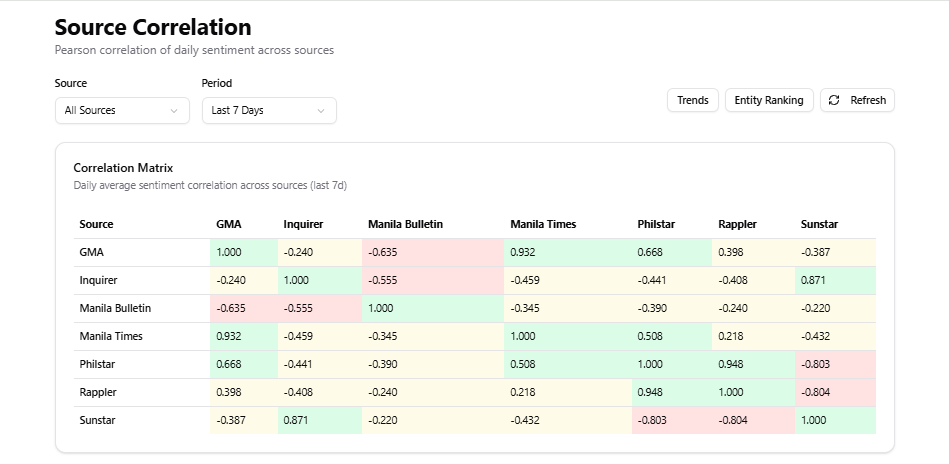
\includegraphics[width=\linewidth]{source-correlation-heatmap.png}}
    \caption{Cross-source sentiment correlation heatmap (Pearson $r$) computed from daily average sentiment scores.}
    \label{fig:correlation-heatmap}
  \end{subfigure}

  \medskip

  \begin{subfigure}{0.49\linewidth}
    \centering
    \imgbox{\includegraphics[width=\linewidth]{GMA.png}}
    \caption{GMA daily average VADER sentiment.}
    \label{fig:correlation-gma}
  \end{subfigure}
  \hfill
  \begin{subfigure}{0.49\linewidth}
    \centering
    \imgbox{\includegraphics[width=\linewidth]{Manila_Times.png}}
    \caption{Manila Times daily average VADER sentiment.}
    \label{fig:correlation-mt}
  \end{subfigure}

  \caption{Correlation and outlet-level sentiment summaries for the observation window (Feb.~28--Mar.~6; Feb.~28 partial due to a power interruption).}
  \label{fig:correlation}
\end{figure}

As shown in Figure~\ref{fig:correlation-heatmap}, the correlation matrix presents the pairwise Pearson correlation coefficients of daily average sentiment scores across the seven news sources over the observation window (Feb.~28--Mar.~6). The values range from $-1$ to $1$, where $1$ indicates perfect positive correlation, $-1$ indicates perfect negative correlation, and $0$ indicates no linear association. Data for Feb.~28 is incomplete due to a city power interruption during collection; Manila Times collected 8 articles while GMA collected none, so Feb.~28 is treated as partial coverage in the per-source comparisons below.

The matrix reveals several notable patterns. For instance, GMA and Manila Times exhibit a strong positive correlation of $0.932$, suggesting that these sources tend to report news with similar sentiment trends during the observed period.

Some correlations may reflect reporting focus or editorial tone. For example, Rappler and Philstar display a high positive correlation ($0.948$), which could indicate synchronized coverage on certain national events, while GMA and Inquirer show a negative correlation ($-0.240$), suggesting occasional divergence in reporting sentiment.

It is important to note that these correlations do not imply causation or editorial bias; rather, they provide a quantitative measure of how the sentiment patterns of different sources fluctuate together. This analysis allows researchers to identify clusters of media outlets with similar reporting behavior and to explore patterns in how news sentiment evolves across the Philippine media landscape over time.

\textbf{GMA average sentiment.} Table}
  \centering
  \small
  \begin{tabular}{lr}
    \toprule
    Date & VADER average score \\
    \midrule
    Feb. 28 & N/A (0 articles) \\
    March 1 & 0.077 \\
    March 2 & -0.165 \\
    March 3 & 0.097 \\
    March 4 & 0.104 \\
    March 5 & 0.076 \\
    March 6 & 0.042 \\
    \bottomrule
  \end{tabular}
\end{table}

\textbf{Manila Times average sentiment.} Table~\ref{tab:manilatimes-avg} lists the daily VADER average score for Manila Times (see Figure~\ref{fig:correlation}(\subref{fig:correlation-mt})).
\begin{table}[h]
  \caption{Manila Times daily average sentiment (VADER).}
  \label{tab:manilatimes-avg}
  \centering
  \small
  \begin{tabular}{lr}
    \toprule
    Date & VADER average score \\
    \midrule
    Feb. 28 & N/A (8 articles; power interruption) \\
    March 1 & 0.351 \\
    March 2 & 0.145 \\
    March 3 & 0.523 \\
    March 4 & 0.409 \\
    March 5 & 0.441 \\
    March 6 & 0.267 \\
    \bottomrule
  \end{tabular}
\end{table}

\textbf{Movement direction comparison.} Table~\ref{tab:gma-mt-movement} summarizes whether both outlets move in the same direction each day.
\begin{table}[h]
  \caption{Movement direction comparison (GMA vs.\ Manila Times).}
  \label{tab:gma-mt-movement}
  \centering
  \small
  \begin{tabular}{p{0.22\columnwidth}p{0.22\columnwidth}p{0.30\columnwidth}p{0.16\columnwidth}}
    \toprule
    Date & GMA & Manila Times & Result \\
    \midrule
    Feb. 28 & N/A (0 articles) & N/A (8 articles) & N/A \\
    March 1 & $\uparrow$ positive score & $\uparrow$ positive score & match \\
    March 2 & $\downarrow$ drop score & $\downarrow$ drop score & match \\
    March 3 & $\uparrow$ rise score & $\uparrow$ rise score & match \\
    March 4 & $\uparrow$ rise score & $\uparrow$ rise score & match \\
    March 5 & $\rightarrow$ stable & $\rightarrow$ stable & match \\
    March 6 & $\downarrow$ drop score & $\downarrow$ drop score & match \\
    \bottomrule
  \end{tabular}
\end{table}

\textbf{Relationship between GMA and Manila Times.} Figure~\ref{fig:correlation} reveals a very strong positive relationship between GMA and Manila Times ($r=0.932$). This indicates that the daily sentiment patterns of the two outlets move in a highly synchronized manner during the observation period. Although the overall sentiment distribution differs---where Manila Times exhibits a substantially higher proportion of positive articles (70.6\%) compared to GMA (52\%)---both sources demonstrate similar directional changes in sentiment across the same days (Tables~\ref{tab:gma-avg}--\ref{tab:gma-mt-movement}). For example, both outlets exhibit a noticeable drop in sentiment on March 2 followed by a consistent rise between March 3 and March 4 before stabilizing toward the end of the observation window. This pattern suggests that the outlets may be responding to similar news cycles or events during the period analyzed. However, the correlation should be interpreted strictly as a statistical relationship rather than evidence of editorial alignment or influence.

\textbf{Note.} This correlation reflects statistical association only and should not be interpreted as evidence of editorial influence. Model limitations (e.g., VADER’s handling of context) may also affect sentiment interpretation.
\subsection{Most Frequent Entities and Their Sentiment Profiles}
Figure~\ref{fig:entities} presents the most frequently mentioned named entities extracted from the collected news articles, along with their corresponding average sentiment scores. The ranking highlights the most visible actors within the observation window and summarizes the overall tone associated with their coverage.

\begin{figure}[h]
  \centering
  \imgbox{\includegraphics[width=\linewidth]{entities_chart.png}}
  \caption{Top mentioned entities with average sentiment scores.}
  \label{fig:entities}
\end{figure}

The results show a strong dominance of political actors and government institutions in the dataset. The most frequently mentioned entity is Duterte, appearing 360 times with a strongly negative average sentiment score ($-0.727$), indicating that coverage during the observation period is largely associated with unfavorable or critical reporting. This reflects how high-profile political figures tend to attract sentiment-polarized narratives in news media.

Other political figures, including Sara Duterte and Ferdinand Marcos Jr., also appear prominently, together with institutional entities such as the Senate of the Philippines, the House of Representatives of the Philippines, and the Supreme Court of the Philippines. This concentration suggests that the news cycle during the selected period is heavily centered on governance, policy, and legal developments.

In contrast, international entities such as the United States and the Middle East appear with sentiment scores closer to neutral, though still slightly negative. This pattern may reflect the nature of international reporting, which often emphasizes geopolitical tensions, conflicts, or security-related issues rather than purely positive developments.

Overall, the entity-level analysis demonstrates the system’s ability to identify influential actors and associate them with aggregated sentiment signals. Beyond frequency counts, this approach provides a structured way to examine how different entities are portrayed in the media, enabling deeper investigation into potential bias, framing, or narrative trends across news sources.

\section{Conclusion}
This study successfully designed and implemented PH Eye, an automated media sentiment monitoring system for Philippine online news. The platform integrates scheduled web scraping, text normalization, sentiment scoring, and named entity extraction, and presents results through interactive analytics for trend monitoring and cross-source comparison.

The system can continuously collect and process articles from multiple outlets, persisting normalized article records, sentiment outputs, and scraping logs in a relational database to ensure traceability and reproducible aggregation. As of March 17, 2026, the deployed pipeline has ingested 26,510 articles, demonstrating that the architecture is capable of ongoing collection and analysis for future research. Quantitative results reported in this paper are based on a 7-day snapshot, selected to represent the period of most consistent uninterrupted system operation during evaluation.

PH Eye supports sentiment trend summaries, cross-source correlation analysis, and entity-level aggregation, illustrating how statistical summaries and text mining can combine to reveal patterns in large-scale news streams. These outputs serve as exploratory indicators to guide deeper qualitative review rather than definitive judgments of intent or bias.

\textbf{Limitations.} This study is subject to several limitations. The reliance on VADER, a lexicon-based sentiment model, may result in misinterpretation of sarcasm, domain-specific language, and context-dependent polarity. While chunked scoring and weighted aggregation help mitigate long-document dilution, the resulting sentiment scores should be interpreted as indicative rather than definitive. Furthermore, scraper downtime and website layout changes may introduce missing data or uneven source coverage within the observation window. Additionally, it was observed that SunStar occasionally publishes content in Cebuano, which may introduce noise, as VADER is primarily optimized for English. This limitation highlights the need for multilingual or transformer-based sentiment models in future work to better handle mixed-language corpora.

\section{Recommendations and Artifact Availability}

\subsection{Recommendations}
\begin{itemize}
    \item \textbf{Benchmark Dataset:} Construct a manually labeled Philippine news sentiment dataset to enable objective evaluation, calibrate sentiment thresholds locally, and support more defensible performance reporting.
    \item \textbf{Entity Normalization:} Improve entity normalization to reduce ambiguity across aliases, acronyms, and geopolitical variants, increasing reliability of entity-level summaries.
    \item \textbf{Data Quality Audits:} Implement periodic audits to quantify scraper coverage, detect missing days, and identify source-specific failures early via automated monitoring.
    \item \textbf{Transformer-based NLP:} Explore transformer-based NLP models as an optional high-accuracy mode for complex linguistic cases, while retaining VADER for near real-time processing on limited compute resources.
    \item \textbf{Flexible Date-range Filtering:} Extend the platform with explicit date-range filtering beyond fixed 7-day and 30-day windows, supporting reproducible experimental windows and comparative studies across historical periods.
\end{itemize}

\subsection{Artifact / Source Code Availability}
To support reproducibility, the PH Eye source code and evaluation scripts are publicly available on GitHub \cite{pheye_github}. The repository includes build/run instructions and a pinned version corresponding to the system configuration used for the reported snapshot. Due to copyright and licensing constraints of publisher content, the study does not redistribute full article text; instead, it provides the software pipeline, database schemas, and aggregated outputs necessary to replicate the analysis on newly collected data.

\begin{acks}
The author thanks Dr.\ Lea P.\ Ymalay and Guimaras State University for guidance and support during this capstone project.
\end{acks}

\bibliographystyle{ACM-Reference-Format}
\bibliography{references}

\end{document}
